% Options for packages loaded elsewhere
\PassOptionsToPackage{unicode}{hyperref}
\PassOptionsToPackage{hyphens}{url}
%
\documentclass[
  11pt,
]{article}
\usepackage[]{mathpazo}
\usepackage{amssymb,amsmath}
\usepackage{ifxetex,ifluatex}
\ifnum 0\ifxetex 1\fi\ifluatex 1\fi=0 % if pdftex
  \usepackage[T1]{fontenc}
  \usepackage[utf8]{inputenc}
  \usepackage{textcomp} % provide euro and other symbols
\else % if luatex or xetex
  \usepackage{unicode-math}
  \defaultfontfeatures{Scale=MatchLowercase}
  \defaultfontfeatures[\rmfamily]{Ligatures=TeX,Scale=1}
\fi
% Use upquote if available, for straight quotes in verbatim environments
\IfFileExists{upquote.sty}{\usepackage{upquote}}{}
\IfFileExists{microtype.sty}{% use microtype if available
  \usepackage[]{microtype}
  \UseMicrotypeSet[protrusion]{basicmath} % disable protrusion for tt fonts
}{}
\makeatletter
\@ifundefined{KOMAClassName}{% if non-KOMA class
  \IfFileExists{parskip.sty}{%
    \usepackage{parskip}
  }{% else
    \setlength{\parindent}{0pt}
    \setlength{\parskip}{6pt plus 2pt minus 1pt}}
}{% if KOMA class
  \KOMAoptions{parskip=half}}
\makeatother
\usepackage{xcolor}
\IfFileExists{xurl.sty}{\usepackage{xurl}}{} % add URL line breaks if available
\IfFileExists{bookmark.sty}{\usepackage{bookmark}}{\usepackage{hyperref}}
\hypersetup{
  pdftitle={Trabajo final Estadística Avanzada},
  pdfkeywords={Maestria Ciencia Datos, ,},
  hidelinks,
  pdfcreator={LaTeX via pandoc}}
\urlstyle{same} % disable monospaced font for URLs
\usepackage[margin=1in]{geometry}
\usepackage{color}
\usepackage{fancyvrb}
\newcommand{\VerbBar}{|}
\newcommand{\VERB}{\Verb[commandchars=\\\{\}]}
\DefineVerbatimEnvironment{Highlighting}{Verbatim}{commandchars=\\\{\}}
% Add ',fontsize=\small' for more characters per line
\usepackage{framed}
\definecolor{shadecolor}{RGB}{248,248,248}
\newenvironment{Shaded}{\begin{snugshade}}{\end{snugshade}}
\newcommand{\AlertTok}[1]{\textcolor[rgb]{0.94,0.16,0.16}{#1}}
\newcommand{\AnnotationTok}[1]{\textcolor[rgb]{0.56,0.35,0.01}{\textbf{\textit{#1}}}}
\newcommand{\AttributeTok}[1]{\textcolor[rgb]{0.77,0.63,0.00}{#1}}
\newcommand{\BaseNTok}[1]{\textcolor[rgb]{0.00,0.00,0.81}{#1}}
\newcommand{\BuiltInTok}[1]{#1}
\newcommand{\CharTok}[1]{\textcolor[rgb]{0.31,0.60,0.02}{#1}}
\newcommand{\CommentTok}[1]{\textcolor[rgb]{0.56,0.35,0.01}{\textit{#1}}}
\newcommand{\CommentVarTok}[1]{\textcolor[rgb]{0.56,0.35,0.01}{\textbf{\textit{#1}}}}
\newcommand{\ConstantTok}[1]{\textcolor[rgb]{0.00,0.00,0.00}{#1}}
\newcommand{\ControlFlowTok}[1]{\textcolor[rgb]{0.13,0.29,0.53}{\textbf{#1}}}
\newcommand{\DataTypeTok}[1]{\textcolor[rgb]{0.13,0.29,0.53}{#1}}
\newcommand{\DecValTok}[1]{\textcolor[rgb]{0.00,0.00,0.81}{#1}}
\newcommand{\DocumentationTok}[1]{\textcolor[rgb]{0.56,0.35,0.01}{\textbf{\textit{#1}}}}
\newcommand{\ErrorTok}[1]{\textcolor[rgb]{0.64,0.00,0.00}{\textbf{#1}}}
\newcommand{\ExtensionTok}[1]{#1}
\newcommand{\FloatTok}[1]{\textcolor[rgb]{0.00,0.00,0.81}{#1}}
\newcommand{\FunctionTok}[1]{\textcolor[rgb]{0.00,0.00,0.00}{#1}}
\newcommand{\ImportTok}[1]{#1}
\newcommand{\InformationTok}[1]{\textcolor[rgb]{0.56,0.35,0.01}{\textbf{\textit{#1}}}}
\newcommand{\KeywordTok}[1]{\textcolor[rgb]{0.13,0.29,0.53}{\textbf{#1}}}
\newcommand{\NormalTok}[1]{#1}
\newcommand{\OperatorTok}[1]{\textcolor[rgb]{0.81,0.36,0.00}{\textbf{#1}}}
\newcommand{\OtherTok}[1]{\textcolor[rgb]{0.56,0.35,0.01}{#1}}
\newcommand{\PreprocessorTok}[1]{\textcolor[rgb]{0.56,0.35,0.01}{\textit{#1}}}
\newcommand{\RegionMarkerTok}[1]{#1}
\newcommand{\SpecialCharTok}[1]{\textcolor[rgb]{0.00,0.00,0.00}{#1}}
\newcommand{\SpecialStringTok}[1]{\textcolor[rgb]{0.31,0.60,0.02}{#1}}
\newcommand{\StringTok}[1]{\textcolor[rgb]{0.31,0.60,0.02}{#1}}
\newcommand{\VariableTok}[1]{\textcolor[rgb]{0.00,0.00,0.00}{#1}}
\newcommand{\VerbatimStringTok}[1]{\textcolor[rgb]{0.31,0.60,0.02}{#1}}
\newcommand{\WarningTok}[1]{\textcolor[rgb]{0.56,0.35,0.01}{\textbf{\textit{#1}}}}
\usepackage{graphicx,grffile}
\makeatletter
\def\maxwidth{\ifdim\Gin@nat@width>\linewidth\linewidth\else\Gin@nat@width\fi}
\def\maxheight{\ifdim\Gin@nat@height>\textheight\textheight\else\Gin@nat@height\fi}
\makeatother
% Scale images if necessary, so that they will not overflow the page
% margins by default, and it is still possible to overwrite the defaults
% using explicit options in \includegraphics[width, height, ...]{}
\setkeys{Gin}{width=\maxwidth,height=\maxheight,keepaspectratio}
% Set default figure placement to htbp
\makeatletter
\def\fps@figure{htbp}
\makeatother
\setlength{\emergencystretch}{3em} % prevent overfull lines
\providecommand{\tightlist}{%
  \setlength{\itemsep}{0pt}\setlength{\parskip}{0pt}}
\setcounter{secnumdepth}{-\maxdimen} % remove section numbering
\usepackage[]{natbib}
\bibliographystyle{apsr}

\title{Trabajo final Estadística Avanzada}
\author{true \and true \and true \and true}
\date{octubre 28, 2020}

\begin{document}
\maketitle
\begin{abstract}
Este documento anliza los impactos de las variables macoreconómicas en
los costos y gastos de una empresa en un determinado sector económico
\end{abstract}

{
\setcounter{tocdepth}{3}
\tableofcontents
}
\{newpage\}

\hypertarget{capuxedtulo-1-lectura-de-variables-de-empresa}{%
\section{Capítulo 1 Lectura de variables de
empresa}\label{capuxedtulo-1-lectura-de-variables-de-empresa}}

Actividad de evaluación de la asignatura Métodos Estadísticos Avanzados
Profesor: Juan David Ospina Arango Estudiantes: Cindy Guerra, Diana
Benjumea, Carlos Murillo, Luz Florez

Métodos Estadísticos Avanzados Maestría en Ciencia de los Datos
Universidad EAFIT

Objetivo Caracterizar las relaciones entre algunos indicadores
macroeconómicos y los costos y gastos de ventas de las empresas
colombianas vigiladas por la SuperSociedades.

Lineamientos: 1. Con ayuda de un modelo lineal modele cree un modelo o
varios modelos que permitan caracterizar la relación entre las variables
PIB, Inflación, Desempleo, Tasa de Cambio, Balance Fiscal, Balance en
Cuenta Corriente, Tasa de intervención, TRM y los costos y gastos de
ventas.

\begin{enumerate}
\def\labelenumi{\arabic{enumi}.}
\setcounter{enumi}{1}
\item
  Se debe escoger mínimo un tipo de empresas (Clasificación Industrial
  Internacional Uniforme) que tenga más de 20 empresas y tomar al menos
  los últimos tres años de información disponible.
\item
  Se debe evaluar el ajuste y la capacidad predictiva.
\item
  Se deben explicar todas las transformaciones de variables requeridas
  por el modelo.
\item
  Se deben explicar todos los pasos para la construcción de la base de
  datos: descarga de información, concatenación, etc.
\item
  Se debe incluir un análisis descriptivo.
\item
  Se debe incluir un análsis de la razonabilidad de las cifras.
\item
  Se debe redactar un reporte técnico documentando lo anterior. La
  sugerencia es utilizar un formato que permita la inclusión de gráficos
  basados en html o JavaScript (por ejemplo hmtl a partir de Rmarkdown).
  El código se debe subir a un repositorio Git y referenciarlo en el
  reporte. El reporte debe incluir una estimación del esfuerzo de las
  actividades de 1) consolidación de información, 3) transformación de
  varibles y análisis descriptivo, 4) ajuste y validación de modelos y
  5) redacción del reporte.
\item
  El trabajo se debe subir al canal del curso en Teams y se debe
  notificar por correo a la dirección
  \href{mailto:judaospi@bancolombia.com.co}{\nolinkurl{judaospi@bancolombia.com.co}}.
\item
  La fecha de entrega es el viernes 30 de octubre y el trabajo se puede
  presentar en equipos de máximo cinco estudiantes.
\end{enumerate}

Para acceder a los datos de costos y gastos de ventas: • Entrar a
\url{http://pie.supersociedades.gov.co} \textgreater{} MENÚ
\textgreater{} Descarga Masiva de Información Descargar la información
de los años 2016 a 2019

Primera iteración: Código CIIU seleccionado: G4711 Macrosector: Comercio
Descripción: Comercio al por menor en establecimientos no especializados
con surtido compuesto principalmente por alimentos, bebidas o tabaco.

Esta clase incluye: • Los establecimientos no especializados de comercio
al por menor de productos cuyo surtido está compuesto principalmente de
alimentos (víveres en general), bebidas o tabaco. No obstante, expenden
otras mercancías para consumo de los hogares tales como vestuario,
electrodomésticos, muebles, artículos de ferretería, cosméticos, entre
otros. Suelen realizar este tipo de actividad los denominados
supermercados, cooperativas de consumidores, comisariatos y otros
establecimientos similares. También se incluyen las tiendas, los
graneros, entre otros, que se encuentran en los pueblos o en barrios
tradicionales.

Esta clase excluye: • El expendio de comidas preparadas en restaurantes,
cafeterías y por autoservicio.

Al realizar los cargues iniciales de información nos dimos cuenta de que
nos cruzaban muy pocas empresas porlo que el conjunto de datos
seleccionado no era suficiente.

Iteración 2: Código CIIU seleccionado: B0722

\begin{Shaded}
\begin{Highlighting}[]
\KeywordTok{library}\NormalTok{(tidyverse)}
\KeywordTok{library}\NormalTok{(}\StringTok{"readxl"}\NormalTok{)}
\KeywordTok{library}\NormalTok{(}\StringTok{"dplyr"}\NormalTok{)}
\end{Highlighting}
\end{Shaded}

\begin{enumerate}
\def\labelenumi{\arabic{enumi}.}
\tightlist
\item
  Cargamos los datos básicos de las empresas
\end{enumerate}

\begin{Shaded}
\begin{Highlighting}[]
\CommentTok{#Revisamos como son nuestros datos para saber si tenemos que realizar algún ajuste a la carga}
\KeywordTok{file.show}\NormalTok{(}\StringTok{"./data/datosBasicosComplete.xlsx"}\NormalTok{)}

\CommentTok{#Como el archivo no tiene forma de tabla al principio, debemos realizar la carga, ignorando las primeras filas del archivo.}

\CommentTok{#Cargar los archivos a un dataframe}
\NormalTok{pd_datos_basicos <-}\StringTok{ }\KeywordTok{read_excel}\NormalTok{(}\StringTok{"./data/datosBasicosComplete.xlsx"}\NormalTok{, }\DataTypeTok{sheet =} \StringTok{"Reporte"}\NormalTok{, }\DataTypeTok{skip=}\DecValTok{8}\NormalTok{, }\DataTypeTok{col_types =} \KeywordTok{c}\NormalTok{(}\StringTok{"text"}\NormalTok{, }
\StringTok{"text"}\NormalTok{, }\StringTok{"text"}\NormalTok{, }\StringTok{"text"}\NormalTok{, }\StringTok{"text"}\NormalTok{,}\StringTok{"text"}\NormalTok{,}\StringTok{"text"}\NormalTok{,}\StringTok{"text"}\NormalTok{,}\StringTok{"text"}\NormalTok{, }\StringTok{"text"}\NormalTok{,}\StringTok{"text"}\NormalTok{,}\StringTok{"text"}\NormalTok{,}\StringTok{"text"}\NormalTok{,}\StringTok{"text"}\NormalTok{,}\StringTok{"text"}\NormalTok{,}\StringTok{"text"}\NormalTok{,}\StringTok{"date"}\NormalTok{,}
\StringTok{"text"}\NormalTok{,}\StringTok{"date"}\NormalTok{,}\StringTok{"text"}\NormalTok{,}\StringTok{"date"}\NormalTok{, }\StringTok{"text"}\NormalTok{, }\StringTok{"text"}\NormalTok{))}

\NormalTok{pd_datos_basicos }\OperatorTok\StringTok{ }\KeywordTok{mutate}\NormalTok{(}\StringTok{`}\DataTypeTok{Órgano Societario}\StringTok{`}\NormalTok{ =}\StringTok{ }\KeywordTok{as.factor}\NormalTok{(}\StringTok{`}\DataTypeTok{Órgano Societario}\StringTok{`}\NormalTok{),}
                            \StringTok{`}\DataTypeTok{Etapa Situación` = as.factor(}\StringTok{`}\NormalTok{Etapa Situación`)}\ErrorTok{)}\NormalTok{ ->}\StringTok{ }\NormalTok{pd_datos_basicos}

\KeywordTok{head}\NormalTok{(pd_datos_basicos)}
\end{Highlighting}
\end{Shaded}

\begin{verbatim}
## # A tibble: 6 x 23
##   NIT   `Razón social` `Código CIIU` `Tipo Societari~ `Objeto Social`
##   <chr> <chr>          <chr>         <chr>            <chr>          
## 1 1001~ NOREÑA  MANRI~ 0             PERSONA NATURAL  <NA>           
## 2 1001~ PEÑA RAMIREZ ~ H5229         PERSONA NATURAL  <NA>           
## 3 1002~ GONZALEZ SANC~ G4731         PERSONA NATURAL  <NA>           
## 4 1002~ RODRIGO JAVIE~ L6810         PERSONA NATURAL  <NA>           
## 5 1002~ BUITRAGO GONZ~ H4923         PERSONA NATURAL  <NA>           
## 6 1005~ KAREN JULIETH~ M7500         PERSONA NATURAL  <NA>           
## # ... with 18 more variables: `Dirección Notificación Judicial` <chr>, `Ciudad
## #   Notificación Judicial` <chr>, `Departamento Notificación Judicial` <chr>,
## #   `Teléfono Notificación Judicial` <chr>, `Dirección Domicilio` <chr>,
## #   `Ciudad Domicilio` <chr>, `Departamento Domicilio` <chr>, `Apartado
## #   Domicilio` <chr>, `E-Mail` <chr>, Web <chr>, Estado <chr>, `Fecha
## #   Estado` <dttm>, Situación <chr>, `Fecha Situación` <dttm>, `Etapa
## #   Situación` <fct>, `Fecha Etapa` <dttm>, `Nombre Representante Legal` <chr>,
## #   `Órgano Societario` <fct>
\end{verbatim}

\begin{Shaded}
\begin{Highlighting}[]
\KeywordTok{library}\NormalTok{(dplyr)}

\NormalTok{pd_datos_basicos_flt <-}\StringTok{ }\NormalTok{pd_datos_basicos[,}\KeywordTok{c}\NormalTok{(}\StringTok{"NIT"}\NormalTok{,}\StringTok{"Razón social"}\NormalTok{,}\StringTok{"Código CIIU"}\NormalTok{,}\StringTok{"Ciudad Domicilio"}\NormalTok{,}\StringTok{"Departamento Domicilio"}\NormalTok{, }\StringTok{"Estado"}\NormalTok{,}\StringTok{"Situación", "}\NormalTok{Órgano Societario}\StringTok{", "}\NormalTok{Etapa Situación")]}

\KeywordTok{names}\NormalTok{ (pd_datos_basicos_flt) =}\StringTok{ }\KeywordTok{c}\NormalTok{(}\StringTok{"NIT"}\NormalTok{,}\StringTok{"razon_social"}\NormalTok{,}\StringTok{"CIIU"}\NormalTok{,}\StringTok{"ciudad"}\NormalTok{,}\StringTok{"departamento"}\NormalTok{, }\StringTok{"estado"}\NormalTok{,}\StringTok{"situacion"}\NormalTok{, }\StringTok{"organo_societario"}\NormalTok{,}
                                 \StringTok{"etapa_situacion"}\NormalTok{)}

\NormalTok{pd_datos_basicos_flt <-}\StringTok{ }\KeywordTok{filter}\NormalTok{(pd_datos_basicos_flt, CIIU }\OperatorTok{==}\StringTok{ "B0722"} \OperatorTok{&}\StringTok{ }\NormalTok{situacion }\OperatorTok{==}\StringTok{ "ACTIVA"}\NormalTok{)}

\KeywordTok{head}\NormalTok{(pd_datos_basicos_flt)}
\end{Highlighting}
\end{Shaded}

\begin{verbatim}
## # A tibble: 6 x 9
##   NIT   razon_social CIIU  ciudad departamento estado situacion organo_societar~
##   <chr> <chr>        <chr> <chr>  <chr>        <chr>  <chr>     <fct>           
## 1 8002~ GRUPO DE BU~ B0722 MEDEL~ ANTIOQUIA    INSPE~ ACTIVA    ACTIVIDAD ECONO~
## 2 8110~ MINERA CROE~ B0722 MEDEL~ ANTIOQUIA    INSPE~ ACTIVA    ACTIVIDAD ECONO~
## 3 8110~ NUEVA CALIF~ B0722 MEDEL~ ANTIOQUIA    INSPE~ ACTIVA    ACTIVIDAD ECONO~
## 4 8110~ COLOMBIA GO~ B0722 MEDEL~ ANTIOQUIA    INSPE~ ACTIVA    ACTIVIDAD ECONO~
## 5 8110~ NEGOCIOS MI~ B0722 MEDEL~ ANTIOQUIA    INSPE~ ACTIVA    ACTIVIDAD ECONO~
## 6 8300~ ECO ORO MIN~ B0722 BUCAR~ SANTANDER    INSPE~ ACTIVA    ACTIVIDAD ECONO~
## # ... with 1 more variable: etapa_situacion <fct>
\end{verbatim}

\begin{enumerate}
\def\labelenumi{\arabic{enumi}.}
\setcounter{enumi}{2}
\tightlist
\item
  Cargamos los datos financieros
\end{enumerate}

\begin{Shaded}
\begin{Highlighting}[]
\NormalTok{pd_datos_fin_}\DecValTok{2017}\NormalTok{ <-}\StringTok{ }\KeywordTok{read_excel}\NormalTok{(}\StringTok{"./data/Plenas - Individuales2017.xlsx"}\NormalTok{, }\DataTypeTok{sheet =} \StringTok{"Estado de Resultado Integral"}\NormalTok{ )}

\NormalTok{pd_datos_fin_}\DecValTok{2017}\NormalTok{ <-}\StringTok{ }\NormalTok{pd_datos_fin_}\DecValTok{2017}\NormalTok{[,}\KeywordTok{c}\NormalTok{(}\StringTok{"Nit"}\NormalTok{, }\StringTok{"Periodo"}\NormalTok{, }\StringTok{"Costo de ventas"}\NormalTok{,  }\StringTok{"Costos de distribución", "}\NormalTok{Gastos de administración", }\StringTok{"Otros gastos, por función", "}\NormalTok{Costos financieros}\StringTok{", "}\KeywordTok{Gasto}\NormalTok{ (ingreso) por impuestos, operaciones continuadas}\StringTok{", "}\NormalTok{Ingresos de actividades ordinarias}\StringTok{", "}\NormalTok{Otros ingresos}\StringTok{", "}\NormalTok{Ingresos financieros}\StringTok{")]}

\StringTok{names (pd_datos_fin_2017) = c("}\NormalTok{NIT}\StringTok{", "}\NormalTok{Periodo}\StringTok{", "}\NormalTok{costo_ventas}\StringTok{",  "}\NormalTok{costo_distribucion}\StringTok{", "}\NormalTok{gastos_administracion}\StringTok{", "}\NormalTok{otros_gastos}\StringTok{", "}\NormalTok{costos_financieros}\StringTok{", "}\NormalTok{gasto_impuestos_operaciones}\StringTok{", "}\NormalTok{ingresos_actividades_ordinarias}\StringTok{", "}\NormalTok{otros_ingresos}\StringTok{", "}\NormalTok{ingresos_financieros}\StringTok{")}


\StringTok{datos_completos_fin <- merge (pd_datos_basicos_flt, pd_datos_fin_2017, by.x="}\NormalTok{NIT}\StringTok{", by.y="}\NormalTok{NIT}\StringTok{")}
\end{Highlighting}
\end{Shaded}

Para efectos del ejercicio, no tomaremos el archivo de 2017, ya que el
archivo 2018 tiene los datos de 2017 con la nueva norma.

\begin{Shaded}
\begin{Highlighting}[]
\NormalTok{pd_datos_fin_}\DecValTok{2018}\NormalTok{ <-}\StringTok{ }\KeywordTok{read_excel}\NormalTok{(}\StringTok{"./data/Plenas - Individuales2018.xlsx"}\NormalTok{, }\DataTypeTok{sheet =} \StringTok{"ERI"}\NormalTok{ )}

\NormalTok{pd_datos_fin_}\DecValTok{2018}\NormalTok{ <-}\StringTok{ }\NormalTok{pd_datos_fin_}\DecValTok{2018}\NormalTok{[,}\KeywordTok{c}\NormalTok{(}\StringTok{"Nit"}\NormalTok{, }\StringTok{"Periodo"}\NormalTok{, }\StringTok{"Costo de ventas"}\NormalTok{, }\StringTok{"Gastos de ventas"}\NormalTok{, }\StringTok{"Gastos de administración", "}\NormalTok{Otros gastos}\StringTok{", "}\NormalTok{Costos financieros}\StringTok{", "}\KeywordTok{Ingreso}\NormalTok{ (gasto) por impuestos}\StringTok{", "}\NormalTok{Ingresos de actividades ordinarias}\StringTok{", "}\NormalTok{Otros ingresos}\StringTok{", "}\NormalTok{Ingresos financieros}\StringTok{")]}

\StringTok{names (pd_datos_fin_2018) = c("}\NormalTok{NIT}\StringTok{", "}\NormalTok{Periodo}\StringTok{", "}\NormalTok{costo_ventas}\StringTok{", "}\NormalTok{gastos_ventas}\StringTok{", "}\NormalTok{gastos_administracion}\StringTok{", "}\NormalTok{otros_gastos}\StringTok{", "}\NormalTok{costos_financieros}\StringTok{", "}\NormalTok{gasto_impuestos}\StringTok{", "}\NormalTok{ingresos_actividades_ordinarias}\StringTok{", "}\NormalTok{otros_ingresos}\StringTok{", "}\NormalTok{ingresos_financieros}\StringTok{" )}

\StringTok{datos_completos_2018 <- merge (pd_datos_basicos_flt, pd_datos_fin_2018, by.x="}\NormalTok{NIT}\StringTok{", by.y="}\NormalTok{NIT}\StringTok{")}

\StringTok{#Le damos formato a los periodos}

\StringTok{datos_completos_2018$Periodo[datos_completos_2018$Periodo == "}\NormalTok{Periodo Anterior}\StringTok{"] <- "}\DecValTok{2017}\StringTok{"}
\StringTok{datos_completos_2018$Periodo[datos_completos_2018$Periodo == "}\NormalTok{Periodo Actual}\StringTok{"] <- "}\DecValTok{2018}\StringTok{"}
\end{Highlighting}
\end{Shaded}

\begin{Shaded}
\begin{Highlighting}[]
\NormalTok{pd_datos_fin_}\DecValTok{2019}\NormalTok{ <-}\StringTok{ }\KeywordTok{read_excel}\NormalTok{(}\StringTok{"./data/Plenas - Individuales2019.xlsx"}\NormalTok{, }\DataTypeTok{sheet =} \StringTok{"ERI"}\NormalTok{ )}

\CommentTok{#Revisar Costos de distribución}
\NormalTok{pd_datos_fin_}\DecValTok{2019}\NormalTok{ <-}\StringTok{ }\NormalTok{pd_datos_fin_}\DecValTok{2019}\NormalTok{[,}\KeywordTok{c}\NormalTok{(}\StringTok{"Nit"}\NormalTok{, }\StringTok{"Periodo"}\NormalTok{, }\StringTok{"Costo de ventas"}\NormalTok{, }\StringTok{"Gastos de administración", "}\NormalTok{Otros gastos}\StringTok{", "}\NormalTok{Costos financieros}\StringTok{", "}\KeywordTok{Ingreso}\NormalTok{ (gasto) por impuestos}\StringTok{", "}\NormalTok{Ingresos de actividades ordinarias}\StringTok{", "}\NormalTok{Otros ingresos}\StringTok{", "}\NormalTok{Ingresos financieros}\StringTok{")]}

\StringTok{names (pd_datos_fin_2019) = c("}\NormalTok{NIT}\StringTok{", "}\NormalTok{Periodo}\StringTok{", "}\NormalTok{costo_ventas}\StringTok{", "}\NormalTok{gastos_administracion}\StringTok{", "}\NormalTok{otros_gastos}\StringTok{", "}\NormalTok{costos_financieros}\StringTok{", "}\NormalTok{gasto_impuestos}\StringTok{", "}\NormalTok{ingresos_actividades_ordinarias}\StringTok{", "}\NormalTok{otros_ingresos}\StringTok{", "}\NormalTok{ingresos_financieros}\StringTok{" )}

\StringTok{datos_completos <- merge (pd_datos_basicos_flt, pd_datos_fin_2019, by.x="}\NormalTok{NIT}\StringTok{", by.y="}\NormalTok{NIT}\StringTok{")}

\StringTok{datos_completos$Periodo[datos_completos$Periodo == "}\NormalTok{Periodo Actual}\StringTok{"] <- "}\DecValTok{2019}\StringTok{"}

\StringTok{datos_completos <- filter(datos_completos, Periodo == "}\DecValTok{2019}\StringTok{")}
\end{Highlighting}
\end{Shaded}

\begin{Shaded}
\begin{Highlighting}[]
\CommentTok{#Eliminamos variable diferente a 2019}
\NormalTok{datos_completos_}\DecValTok{2018}\NormalTok{ <-}\StringTok{ }\KeywordTok{select}\NormalTok{(datos_completos_}\DecValTok{2018}\NormalTok{, }\OperatorTok{-}\NormalTok{gastos_ventas)}

\CommentTok{#UNimos los 2 dataframes}
\NormalTok{datos_completos =}\StringTok{ }\KeywordTok{rbind}\NormalTok{(datos_completos, datos_completos_}\DecValTok{2018}\NormalTok{)}
\NormalTok{datos_completos }\OperatorTok\StringTok{ }\KeywordTok{mutate}\NormalTok{( }\DataTypeTok{razon_social =} \KeywordTok{as.factor}\NormalTok{(razon_social), }\DataTypeTok{CIIU =} \KeywordTok{as.factor}\NormalTok{(CIIU), }\DataTypeTok{ciudad =} \KeywordTok{as.factor}\NormalTok{(ciudad),}
                          \DataTypeTok{departamento =} \KeywordTok{as.factor}\NormalTok{(departamento), }\DataTypeTok{estado =}\KeywordTok{as.factor}\NormalTok{(estado), }\DataTypeTok{Periodo =} \KeywordTok{as.factor}\NormalTok{(Periodo),}
                          \DataTypeTok{situacion =} \KeywordTok{as.factor}\NormalTok{(situacion)) ->}\StringTok{ }\NormalTok{datos_completos}
\end{Highlighting}
\end{Shaded}

\begin{Shaded}
\begin{Highlighting}[]
\KeywordTok{library}\NormalTok{(ggplot2)}
\KeywordTok{library}\NormalTok{(lme4)}
\end{Highlighting}
\end{Shaded}

\begin{verbatim}
## Warning: package 'lme4' was built under R version 4.0.3
\end{verbatim}

\begin{verbatim}
## Loading required package: Matrix
\end{verbatim}

\begin{verbatim}
## 
## Attaching package: 'Matrix'
\end{verbatim}

\begin{verbatim}
## The following objects are masked from 'package:tidyr':
## 
##     expand, pack, unpack
\end{verbatim}

\begin{Shaded}
\begin{Highlighting}[]
\KeywordTok{summary}\NormalTok{(datos_completos)}
\end{Highlighting}
\end{Shaded}

\begin{verbatim}
##      NIT                                                razon_social    CIIU   
##  Length:82          ANGLOGOLD ASHANTI COLOMBIA S.A.           : 3    B0722:82  
##  Class :character   CALDAS GOLD MARMATO S.A.S.                : 3              
##  Mode  :character   CONTINENTAL GOLD LIMITED SUCURSAL COLOMBIA: 3              
##                     ECO ORO MINERALS CORP                     : 3              
##                     EXPLORACIONES CHAPARRAL COLOMBIA SAS      : 3              
##                     EXPLORACIONES NORTHERN COLOMBIA S.A.S     : 3              
##                     (Other)                                   :64              
##           ciudad          departamento        estado    situacion 
##  BOGOTÁ, D.C.:26   ANTIOQUIA    :44    INSPECCION:41   ACTIVA:82  
##  BUCARAMANGA :12   BOGOTÁ, D. C.:26    VIGILANCIA:41              
##  ENVIGADO    : 2   SANTANDER    :12                               
##  MEDELLÍN    :42                                                  
##                                                                   
##                                                                   
##                                                                   
##                      organo_societario
##  ACTIVIDAD ECONOMICA DIFERENTE:82     
##  ACTIVIDAD DE VIVIENDA        : 0     
##  BOLSA PROD. AGROPECUARIO     : 0     
##  CLUBES DEPORTIVOS            : 0     
##  COMERCIANTE                  : 0     
##  EMPRESA MULTINACIONAL ANDINA : 0     
##  (Other)                      : 0     
##                                etapa_situacion Periodo    costo_ventas      
##  ACTIVA                                :82     2017:28   Min.   :        0  
##  A LIQUIDACION POR ADJUDICACION        : 0     2018:28   1st Qu.:    59760  
##  ACUERDO CONFIRMADO                    : 0     2019:26   Median : 10986154  
##  ACUERDO DE REORGANIZACION EN EJECUCION: 0               Mean   : 47651275  
##  ADMISION                              : 0               3rd Qu.: 39093635  
##  CANCELADA                             : 0               Max.   :408474390  
##  (Other)                               : 0               NA's   :42         
##  gastos_administracion  otros_gastos      costos_financieros
##  Min.   :     1963     Min.   :       2   Min.   :       0  
##  1st Qu.:   256194     1st Qu.:   16748   1st Qu.:   87145  
##  Median :  1099196     Median :  436728   Median : 1288761  
##  Mean   : 15247178     Mean   : 3893153   Mean   : 4145977  
##  3rd Qu.:  7201307     3rd Qu.: 2322578   3rd Qu.: 3418959  
##  Max.   :287863704     Max.   :46689684   Max.   :52689630  
##  NA's   :16            NA's   :13         NA's   :23        
##  gasto_impuestos     ingresos_actividades_ordinarias otros_ingresos    
##  Min.   : -8974634   Min.   :        0               Min.   :       0  
##  1st Qu.:      499   1st Qu.:        0               1st Qu.:   14600  
##  Median :    36788   Median :        0               Median :  106427  
##  Mean   :  6355794   Mean   :100173105               Mean   : 1106485  
##  3rd Qu.:   813045   3rd Qu.: 42815317               3rd Qu.: 1551194  
##  Max.   :131684824   Max.   :954650443               Max.   :11404344  
##  NA's   :24          NA's   :54                      NA's   :20        
##  ingresos_financieros
##  Min.   :       0    
##  1st Qu.:   15028    
##  Median :  251425    
##  Mean   : 2067049    
##  3rd Qu.: 1794058    
##  Max.   :26100695    
##  NA's   :31
\end{verbatim}

\begin{Shaded}
\begin{Highlighting}[]
\CommentTok{#p1=ggplot(datos, aes(y=cd4,x=week,group=patid,colour=trtarm))}
\CommentTok{#p1+geom_line()}
\end{Highlighting}
\end{Shaded}

REFERENCIAS:

\url{https://www.dian.gov.co/ciiu/Documents/Resolucion_000139_21_Nov_2012.pdf}

\url{https://linea.ccb.org.co/descripcionciiu/}

\url{https://siis.ia.supersociedades.gov.co/}

\url{https://www.supersociedades.gov.co/delegatura_aec/Paginas/Base-completa-EF-2019.aspx}

\hypertarget{capuxedtulo-2-lectura-y-consolidaciuxf3n-de-variables-econuxf3micas}{%
\section{Capítulo 2 Lectura y consolidación de variables
económicas}\label{capuxedtulo-2-lectura-y-consolidaciuxf3n-de-variables-econuxf3micas}}

\textbf{A continuación se preseenta el proceso que se ejecutó para generar un dataframe con las variables de PIB, Inflación, Desempleo, Balance Fiscal, Balance en Cuenta Corriente, Tasa de intervención, TRM}

\textbf{Para el PIB:} Es un indicador económico que refleja el valor
monetario de todos los bienes y servicios finales producidos por un país
o región en un determinado periodo de tiempo, normalmente un año. Se
utiliza para medir la riqueza que genera un país.

\begin{Shaded}
\begin{Highlighting}[]
\KeywordTok{library}\NormalTok{(dplyr)}
\CommentTok{#Los datos son tomados de https://datosmacro.expansion.com/pib/colombia}
\CommentTok{# vectores }
\NormalTok{anyo <-}\StringTok{ }\KeywordTok{c}\NormalTok{(}\StringTok{"2016"}\NormalTok{, }\StringTok{"2017"}\NormalTok{, }\StringTok{"2018"}\NormalTok{, }\StringTok{"2019"}\NormalTok{)}
\NormalTok{PIB_M.E. <-}\StringTok{ }\KeywordTok{c}\NormalTok{(}\FloatTok{289.239}\NormalTok{, }\FloatTok{280.249}\NormalTok{, }\FloatTok{275.999}\NormalTok{, }\FloatTok{255.416}\NormalTok{)}
\NormalTok{Var.PIB <-}\StringTok{ }\KeywordTok{c}\NormalTok{(}\FloatTok{3.3}\NormalTok{, }\FloatTok{2.5}\NormalTok{, }\FloatTok{1.4}\NormalTok{, }\FloatTok{2.1}\NormalTok{)}
\CommentTok{#Crear dataframe de vectores}
\NormalTok{PIB <-}\StringTok{ }\KeywordTok{data.frame}\NormalTok{(anyo, PIB_M.E., Var.PIB)}
\KeywordTok{head}\NormalTok{(PIB)}
\end{Highlighting}
\end{Shaded}

\begin{verbatim}
##   anyo PIB_M.E. Var.PIB
## 1 2016  289.239     3.3
## 2 2017  280.249     2.5
## 3 2018  275.999     1.4
## 4 2019  255.416     2.1
\end{verbatim}

\textbf{Para la inflación:} La inflación es un fenómeno que se observa
en la economía de un país y está relacionado con el aumento desordenado
de los precios de la mayor parte de los bienes y servicios que se
comercian en sus mercados, por un periodo de tiempo prolongado.

\begin{Shaded}
\begin{Highlighting}[]
\CommentTok{#Los datos son tomados de https://es.wikipedia.org/wiki/Anexo:Variaci%C3%B3n_de_la_inflaci%C3%B3n_de_Colombia_desde_1946}
\CommentTok{# vectores }
\NormalTok{anyo <-}\StringTok{ }\KeywordTok{c}\NormalTok{(}\StringTok{"2016"}\NormalTok{, }\StringTok{"2017"}\NormalTok{, }\StringTok{"2018"}\NormalTok{, }\StringTok{"2019"}\NormalTok{)}
\NormalTok{Inflacion <-}\StringTok{ }\KeywordTok{c}\NormalTok{(}\FloatTok{5.75}\NormalTok{, }\FloatTok{4.09}\NormalTok{, }\FloatTok{3.18}\NormalTok{, }\FloatTok{3.80}\NormalTok{)}
\CommentTok{#Crear dataframe de vectores}
\NormalTok{Inflacion <-}\StringTok{ }\KeywordTok{data.frame}\NormalTok{(anyo, Inflacion)}
\KeywordTok{head}\NormalTok{(Inflacion)}
\end{Highlighting}
\end{Shaded}

\begin{verbatim}
##   anyo Inflacion
## 1 2016      5.75
## 2 2017      4.09
## 3 2018      3.18
## 4 2019      3.80
\end{verbatim}

\textbf{Para el desempleo:} Es otra de las variables mas importantes de
la macroeconomía, porque afecta directamente el bienestar de las
personas. El desempleo es el porcentaje de la fuerza de trabajo que está
buscando trabajo activamente y que actualmente se encuentra desempleada.

\begin{Shaded}
\begin{Highlighting}[]
\CommentTok{#Los datos son tomados de https://www.dane.gov.co/index.php/estadisticas-por-tema/mercado-laboral/empleo-y-desempleo}
\CommentTok{# vectores }
\NormalTok{anyo <-}\StringTok{ }\KeywordTok{c}\NormalTok{(}\StringTok{"2016"}\NormalTok{, }\StringTok{"2017"}\NormalTok{, }\StringTok{"2018"}\NormalTok{, }\StringTok{"2019"}\NormalTok{)}
\NormalTok{Desempleo <-}\StringTok{ }\KeywordTok{c}\NormalTok{(}\FloatTok{9.2}\NormalTok{, }\FloatTok{9.4}\NormalTok{, }\FloatTok{9.7}\NormalTok{, }\FloatTok{10.5}\NormalTok{)}
\NormalTok{Var.Desempleo <-}\StringTok{ }\KeywordTok{c}\NormalTok{(}\FloatTok{3.36}\NormalTok{, }\FloatTok{1.99}\NormalTok{, }\FloatTok{3.19}\NormalTok{, }\FloatTok{8.25}\NormalTok{)}
\CommentTok{#Crear dataframe de vectores}
\NormalTok{Desempleo <-}\StringTok{ }\KeywordTok{data.frame}\NormalTok{(anyo, Desempleo, Var.Desempleo)}
\KeywordTok{head}\NormalTok{(Desempleo)}
\end{Highlighting}
\end{Shaded}

\begin{verbatim}
##   anyo Desempleo Var.Desempleo
## 1 2016       9.2          3.36
## 2 2017       9.4          1.99
## 3 2018       9.7          3.19
## 4 2019      10.5          8.25
\end{verbatim}

\textbf{Para el balance fiscal:} Es la diferencia entre ingresos y
gastos públicos en un determinado territorio.

\begin{Shaded}
\begin{Highlighting}[]
\CommentTok{#Los datos son tomados de http://www.urf.gov.co/webcenter/portal/EntidadesFinancieras/pages_EntidadesFinancieras/PoliticaFiscal/bgg/balancefiscalgobiernocentral?_afrLoop=6729623401772216&_afrWindowMode=2&Adf-Window-Id=mof7t7k7j&_afrFS=16&_afrMT=screen&_afrMFW=768&_afrMFH=720&_afrMFDW=1536&_afrMFDH=864&_afrMFC=8&_afrMFCI=0&_afrMFM=0&_afrMFR=120&_afrMFG=0&_afrMFS=0&_afrMFO=0}
\CommentTok{# vectores }
\NormalTok{anyo <-}\StringTok{ }\KeywordTok{c}\NormalTok{(}\StringTok{"2016"}\NormalTok{, }\StringTok{"2017"}\NormalTok{, }\StringTok{"2018"}\NormalTok{, }\StringTok{"2019"}\NormalTok{)}
\NormalTok{GNC <-}\StringTok{ }\KeywordTok{c}\NormalTok{(}\OperatorTok{-}\DecValTok{4}\NormalTok{, }\FloatTok{-3.6}\NormalTok{, }\FloatTok{-3.1}\NormalTok{, }\FloatTok{-2.5}\NormalTok{)}
\CommentTok{#Crear dataframe de vectores}
\NormalTok{GNC <-}\StringTok{ }\KeywordTok{data.frame}\NormalTok{(anyo,GNC)}
\KeywordTok{head}\NormalTok{(GNC)}
\end{Highlighting}
\end{Shaded}

\begin{verbatim}
##   anyo  GNC
## 1 2016 -4.0
## 2 2017 -3.6
## 3 2018 -3.1
## 4 2019 -2.5
\end{verbatim}

\textbf{Para el balance en cuenta corriente:} Es el conjunto de
transacciones de intercambio de bienes y servicios, rentas y
transferencias (tanto corrientes como de capital), su saldo determina la
capacidad o necesidad de financiación de un país.

\begin{Shaded}
\begin{Highlighting}[]
\CommentTok{# vectores }
\NormalTok{anyo <-}\StringTok{ }\KeywordTok{c}\NormalTok{(}\StringTok{"2016"}\NormalTok{, }\StringTok{"2017"}\NormalTok{, }\StringTok{"2018"}\NormalTok{, }\StringTok{"2019"}\NormalTok{)}
\NormalTok{Balance_Cuenta_Corriente <-}\StringTok{ }\KeywordTok{c}\NormalTok{(}\OperatorTok{-}\FloatTok{13747.75}\NormalTok{, }\FloatTok{-13117.66}\NormalTok{, }\FloatTok{-10240.88}\NormalTok{, }\FloatTok{-12036.18}\NormalTok{)}
\CommentTok{#Crear dataframe de vectores}
\NormalTok{Balance_Cuenta_Corriente <-}\StringTok{ }\KeywordTok{data.frame}\NormalTok{(anyo, Balance_Cuenta_Corriente)}
\KeywordTok{head}\NormalTok{(Balance_Cuenta_Corriente)}
\end{Highlighting}
\end{Shaded}

\begin{verbatim}
##   anyo Balance_Cuenta_Corriente
## 1 2016                -13747.75
## 2 2017                -13117.66
## 3 2018                -10240.88
## 4 2019                -12036.18
\end{verbatim}

\textbf{Para la tasa de intervención:} Corresponde a la tasa de interés
mínima que le cobra el Banco de la República a las entidades financieras
por los préstamos que les concede generalmente a un día y, además, sirve
como referencia para establecer la tasa de interés máxima que les paga
por recibirles dinero que tengan como excedente.

\begin{Shaded}
\begin{Highlighting}[]
\CommentTok{#Los datos son tomados de https://www.banrep.gov.co/es/estadisticas/tasas-interes-politica-monetaria}

\CommentTok{# vectores }
\NormalTok{anyo <-}\StringTok{ }\KeywordTok{c}\NormalTok{(}\StringTok{"2016"}\NormalTok{, }\StringTok{"2017"}\NormalTok{, }\StringTok{"2018"}\NormalTok{, }\StringTok{"2019"}\NormalTok{)}
\NormalTok{TIM_promedio<-}\StringTok{ }\KeywordTok{c}\NormalTok{(}\FloatTok{7.10}\NormalTok{, }\FloatTok{6.13}\NormalTok{, }\FloatTok{4.35}\NormalTok{, }\FloatTok{4.25}\NormalTok{)}
\CommentTok{#Crear dataframe de vectores}
\NormalTok{TIM <-}\StringTok{ }\KeywordTok{data.frame}\NormalTok{(anyo, TIM_promedio)}
\KeywordTok{head}\NormalTok{(TIM)}
\end{Highlighting}
\end{Shaded}

\begin{verbatim}
##   anyo TIM_promedio
## 1 2016         7.10
## 2 2017         6.13
## 3 2018         4.35
## 4 2019         4.25
\end{verbatim}

\textbf{Para la TRM:} La tasa de cambio representativa del mercado (TRM)
es la cantidad de pesos colombianos por un dólar de los Estados Unidos.
La TRM se calcula con base en las operaciones de compra y venta de
divisas entre intermediarios financieros que transan en el mercado
cambiario colombiano, con cumplimiento el mismo día cuando se realiza la
negociación de las divisas.

Actualmente la Superintendencia Financiera de Colombia es la que calcula
y certifica diariamente la TRM con base en las operaciones registradas
el día hábil inmediatamente anterior.

\begin{Shaded}
\begin{Highlighting}[]
\CommentTok{#Se leen los datos - estos datos son tomados de https://www.dolar-colombia.com/historico}
\NormalTok{dataset =}\StringTok{ }\KeywordTok{read.csv}\NormalTok{(}\StringTok{'./data/TRM.csv'}\NormalTok{, }\DataTypeTok{check.names =} \OtherTok{FALSE}\NormalTok{, }\DataTypeTok{encoding =} \StringTok{"UTF-8"}\NormalTok{, }\DataTypeTok{blank.lines.skip =} \OtherTok{FALSE}\NormalTok{, }\DataTypeTok{dec=}\StringTok{","}\NormalTok{)}

\CommentTok{#se conservam unicamente las columnas de año y TRM}
\NormalTok{df =}\StringTok{ }\NormalTok{dataset[}\DecValTok{1}\NormalTok{]}
\NormalTok{df[}\StringTok{'TRM'}\NormalTok{] =}\StringTok{ }\NormalTok{dataset[}\DecValTok{3}\NormalTok{]}
\NormalTok{df}\OperatorTok{$}\NormalTok{TRM <-}\StringTok{ }\KeywordTok{as.numeric}\NormalTok{(}\KeywordTok{as.character}\NormalTok{(df}\OperatorTok{$}\NormalTok{TRM))}

\CommentTok{#Se agrupa bajo la media}
\NormalTok{media =}\StringTok{ }\NormalTok{df}
\NormalTok{media =}\StringTok{ }\NormalTok{media }\OperatorTok
\StringTok{  }\KeywordTok{group_by}\NormalTok{(media[}\DecValTok{1}\NormalTok{]) }\OperatorTok
\StringTok{  }\KeywordTok{summarise}\NormalTok{(}\KeywordTok{across}\NormalTok{(}\DataTypeTok{.cols =} \KeywordTok{everything}\NormalTok{(), }\DataTypeTok{.fns =}\NormalTok{ mean))}
\end{Highlighting}
\end{Shaded}

\begin{verbatim}
## `summarise()` ungrouping output (override with `.groups` argument)
\end{verbatim}

\begin{Shaded}
\begin{Highlighting}[]
\CommentTok{#para la mediana}
\NormalTok{mediana =}\StringTok{ }\NormalTok{df}
\NormalTok{mediana =}\StringTok{ }\NormalTok{mediana }\OperatorTok
\StringTok{  }\KeywordTok{group_by}\NormalTok{(mediana[}\DecValTok{1}\NormalTok{]) }\OperatorTok
\StringTok{  }\KeywordTok{summarise}\NormalTok{(}\KeywordTok{across}\NormalTok{(}\DataTypeTok{.cols =} \KeywordTok{everything}\NormalTok{(), }\DataTypeTok{.fns =}\NormalTok{ median))}
\end{Highlighting}
\end{Shaded}

\begin{verbatim}
## `summarise()` ungrouping output (override with `.groups` argument)
\end{verbatim}

\begin{Shaded}
\begin{Highlighting}[]
\CommentTok{#Se genera un dataframe con los datos obtenidos}
\NormalTok{df =}\StringTok{ }\NormalTok{media}
\KeywordTok{colnames}\NormalTok{(df)[}\DecValTok{2}\NormalTok{] <-}\StringTok{ 'TRM_media'}
\NormalTok{df[}\StringTok{'TRM_mediana'}\NormalTok{] <-}\StringTok{ }\NormalTok{mediana[}\DecValTok{2}\NormalTok{]}
\NormalTok{df}
\end{Highlighting}
\end{Shaded}

\begin{verbatim}
## # A tibble: 4 x 3
##    Anyo TRM_media TRM_mediana
##   <int>     <dbl>       <dbl>
## 1  2016     3051.       3003.
## 2  2017     2951.       2942.
## 3  2018     2956.       2898.
## 4  2019     3281.       3277.
\end{verbatim}

Se unen los datos en un solo dataframe

\begin{Shaded}
\begin{Highlighting}[]
\NormalTok{df[}\StringTok{'PIB_M.E.'}\NormalTok{] =}\StringTok{ }\NormalTok{PIB[}\DecValTok{2}\NormalTok{]}
\NormalTok{df[}\StringTok{'Var.PIB'}\NormalTok{] =}\StringTok{ }\NormalTok{PIB[}\DecValTok{3}\NormalTok{]}
\NormalTok{df[}\StringTok{'Inflacion'}\NormalTok{] =}\StringTok{ }\NormalTok{Inflacion[}\DecValTok{2}\NormalTok{]}
\NormalTok{df[}\StringTok{'Desempleo'}\NormalTok{] =}\StringTok{ }\NormalTok{Desempleo[}\DecValTok{2}\NormalTok{]}
\NormalTok{df[}\StringTok{'var.Desempleo'}\NormalTok{] =}\StringTok{ }\NormalTok{Desempleo[}\DecValTok{3}\NormalTok{]}
\NormalTok{df[}\StringTok{'GNC'}\NormalTok{] =}\StringTok{ }\NormalTok{GNC[}\DecValTok{2}\NormalTok{]}
\NormalTok{df[}\StringTok{'Balance_Cuenta_Corriente'}\NormalTok{] =}\StringTok{ }\NormalTok{Balance_Cuenta_Corriente[}\DecValTok{2}\NormalTok{]}
\NormalTok{df[}\StringTok{'TIM_promedio'}\NormalTok{] =}\StringTok{ }\NormalTok{TIM[}\DecValTok{2}\NormalTok{]}
\KeywordTok{head}\NormalTok{(df)}
\end{Highlighting}
\end{Shaded}

\begin{verbatim}
## # A tibble: 4 x 11
##    Anyo TRM_media TRM_mediana PIB_M.E. Var.PIB Inflacion Desempleo var.Desempleo
##   <int>     <dbl>       <dbl>    <dbl>   <dbl>     <dbl>     <dbl>         <dbl>
## 1  2016     3051.       3003.     289.     3.3      5.75       9.2          3.36
## 2  2017     2951.       2942.     280.     2.5      4.09       9.4          1.99
## 3  2018     2956.       2898.     276.     1.4      3.18       9.7          3.19
## 4  2019     3281.       3277.     255.     2.1      3.8       10.5          8.25
## # ... with 3 more variables: GNC <dbl>, Balance_Cuenta_Corriente <dbl>,
## #   TIM_promedio <dbl>
\end{verbatim}

\hypertarget{capuxedtulo-3-consolidaciuxf3n-de-la-base}{%
\section{Capítulo 3 Consolidación de la
base}\label{capuxedtulo-3-consolidaciuxf3n-de-la-base}}

En esta sección se unen las dos bases generadas en las fases anteriores
en una sola base

\begin{Shaded}
\begin{Highlighting}[]
\NormalTok{datos_completos}\OperatorTok\KeywordTok{mutate}\NormalTok{(}\DataTypeTok{Periodo=}\KeywordTok{as.numeric}\NormalTok{(}\KeywordTok{as.character}\NormalTok{(Periodo))) }\OperatorTok\StringTok{ }\KeywordTok{inner_join}\NormalTok{(df, }\DataTypeTok{by=}\KeywordTok{c}\NormalTok{(}\StringTok{"Periodo"}\NormalTok{ =}\StringTok{ "Anyo"}\NormalTok{)) }\OperatorTok\StringTok{ }\KeywordTok{replace_na}\NormalTok{(}\KeywordTok{list}\NormalTok{(}\DataTypeTok{costo_ventas =} \DecValTok{0}\NormalTok{, }\DataTypeTok{gastos_administracion =} \DecValTok{0}\NormalTok{,}
                                                                                                                                   \DataTypeTok{otros_gastos=}\DecValTok{0}\NormalTok{, }\DataTypeTok{costos_financieros=}\DecValTok{0}\NormalTok{ , }\DataTypeTok{gasto_impuestos=}\DecValTok{0}\NormalTok{, }\DataTypeTok{ingresos_actividades_ordinarias=}\DecValTok{0}\NormalTok{,}
                                                                                                                                   \DataTypeTok{otros_ingresos =} \DecValTok{0}\NormalTok{, }\DataTypeTok{ingresos_financieros=}\DecValTok{0}\NormalTok{)) ->}\StringTok{ }\NormalTok{datos_completos}
\NormalTok{datos_completos }\OperatorTok\StringTok{ }\KeywordTok{mutate}\NormalTok{(}\DataTypeTok{costos_gastos_totales =}\NormalTok{ gastos_administracion }\OperatorTok{+}\StringTok{ }\NormalTok{otros_gastos }\OperatorTok{+}\NormalTok{gasto_impuestos }\OperatorTok{+}\StringTok{ }\NormalTok{costo_ventas,}
                           \DataTypeTok{ingresos_totales =}\NormalTok{ ingresos_actividades_ordinarias }\OperatorTok{+}\StringTok{ }\NormalTok{ingresos_financieros }\OperatorTok{+}\StringTok{ }\NormalTok{otros_ingresos) ->}\StringTok{ }\NormalTok{base_modelado}
                          \CommentTok{#select(gastos_administracion, -otros_gastos, -gasto_impuestos, -costo_ventas, -otros_ingresos, -ingresos_actividades_ordinarias, -ingresos_financieros) }
\NormalTok{base_modelado <-}\StringTok{ }\KeywordTok{droplevels}\NormalTok{(base_modelado)}
\KeywordTok{summary}\NormalTok{(base_modelado)}
\end{Highlighting}
\end{Shaded}

\begin{verbatim}
##      NIT                                                razon_social    CIIU   
##  Length:82          ANGLOGOLD ASHANTI COLOMBIA S.A.           : 3    B0722:82  
##  Class :character   CALDAS GOLD MARMATO S.A.S.                : 3              
##  Mode  :character   CONTINENTAL GOLD LIMITED SUCURSAL COLOMBIA: 3              
##                     ECO ORO MINERALS CORP                     : 3              
##                     EXPLORACIONES CHAPARRAL COLOMBIA SAS      : 3              
##                     EXPLORACIONES NORTHERN COLOMBIA S.A.S     : 3              
##                     (Other)                                   :64              
##           ciudad          departamento        estado    situacion 
##  BOGOTÁ, D.C.:26   ANTIOQUIA    :44    INSPECCION:41   ACTIVA:82  
##  BUCARAMANGA :12   BOGOTÁ, D. C.:26    VIGILANCIA:41              
##  ENVIGADO    : 2   SANTANDER    :12                               
##  MEDELLÍN    :42                                                  
##                                                                   
##                                                                   
##                                                                   
##                      organo_societario etapa_situacion    Periodo    
##  ACTIVIDAD ECONOMICA DIFERENTE:82      ACTIVA:82       Min.   :2017  
##                                                        1st Qu.:2017  
##                                                        Median :2018  
##                                                        Mean   :2018  
##                                                        3rd Qu.:2019  
##                                                        Max.   :2019  
##                                                                      
##   costo_ventas       gastos_administracion  otros_gastos     
##  Min.   :        0   Min.   :        0     Min.   :       0  
##  1st Qu.:        0   1st Qu.:    15366     1st Qu.:     848  
##  Median :        0   Median :   560711     Median :  120317  
##  Mean   : 23244524   Mean   : 12272119     Mean   : 3275946  
##  3rd Qu.:  6666040   3rd Qu.:  5672411     3rd Qu.: 1736150  
##  Max.   :408474390   Max.   :287863704     Max.   :46689684  
##                                                              
##  costos_financieros gasto_impuestos     ingresos_actividades_ordinarias
##  Min.   :       0   Min.   : -8974634   Min.   :        0              
##  1st Qu.:       0   1st Qu.:        0   1st Qu.:        0              
##  Median :  168546   Median :     2546   Median :        0              
##  Mean   : 2983081   Mean   :  4495562   Mean   : 34205451              
##  3rd Qu.: 2383609   3rd Qu.:   141459   3rd Qu.:        0              
##  Max.   :52689630   Max.   :131684824   Max.   :954650443              
##                                                                        
##  otros_ingresos     ingresos_financieros   TRM_media     TRM_mediana  
##  Min.   :       0   Min.   :       0     Min.   :2951   Min.   :2898  
##  1st Qu.:       0   1st Qu.:       0     1st Qu.:2951   1st Qu.:2898  
##  Median :   36549   Median :    3942     Median :2956   Median :2942  
##  Mean   :  836610   Mean   : 1285604     Mean   :3058   Mean   :3033  
##  3rd Qu.:  601104   3rd Qu.:  850632     3rd Qu.:3281   3rd Qu.:3277  
##  Max.   :11404344   Max.   :26100695     Max.   :3281   Max.   :3277  
##                                                                       
##     PIB_M.E.        Var.PIB        Inflacion       Desempleo     
##  Min.   :255.4   Min.   :1.400   Min.   :3.180   Min.   : 9.400  
##  1st Qu.:255.4   1st Qu.:1.400   1st Qu.:3.180   1st Qu.: 9.400  
##  Median :276.0   Median :2.100   Median :3.800   Median : 9.700  
##  Mean   :270.9   Mean   :1.998   Mean   :3.687   Mean   : 9.851  
##  3rd Qu.:280.2   3rd Qu.:2.500   3rd Qu.:4.090   3rd Qu.:10.500  
##  Max.   :280.2   Max.   :2.500   Max.   :4.090   Max.   :10.500  
##                                                                  
##  var.Desempleo        GNC        Balance_Cuenta_Corriente  TIM_promedio  
##  Min.   :1.990   Min.   :-3.60   Min.   :-13118           Min.   :4.250  
##  1st Qu.:1.990   1st Qu.:-3.60   1st Qu.:-13118           1st Qu.:4.250  
##  Median :3.190   Median :-3.10   Median :-12036           Median :4.350  
##  Mean   :4.385   Mean   :-3.08   Mean   :-11792           Mean   :4.926  
##  3rd Qu.:8.250   3rd Qu.:-2.50   3rd Qu.:-10241           3rd Qu.:6.130  
##  Max.   :8.250   Max.   :-2.50   Max.   :-10241           Max.   :6.130  
##                                                                          
##  costos_gastos_totales ingresos_totales   
##  Min.   :     2869     Min.   :        0  
##  1st Qu.:   528039     1st Qu.:    24364  
##  Median :  4175588     Median :   587346  
##  Mean   : 43288150     Mean   : 36327665  
##  3rd Qu.: 26972121     3rd Qu.:  3698197  
##  Max.   :700560590     Max.   :967119965  
## 
\end{verbatim}

\begin{Shaded}
\begin{Highlighting}[]
\KeywordTok{library}\NormalTok{(visdat)}
\end{Highlighting}
\end{Shaded}

\begin{verbatim}
## Warning: package 'visdat' was built under R version 4.0.3
\end{verbatim}

\begin{Shaded}
\begin{Highlighting}[]
\KeywordTok{vis_miss}\NormalTok{(base_modelado)}
\end{Highlighting}
\end{Shaded}

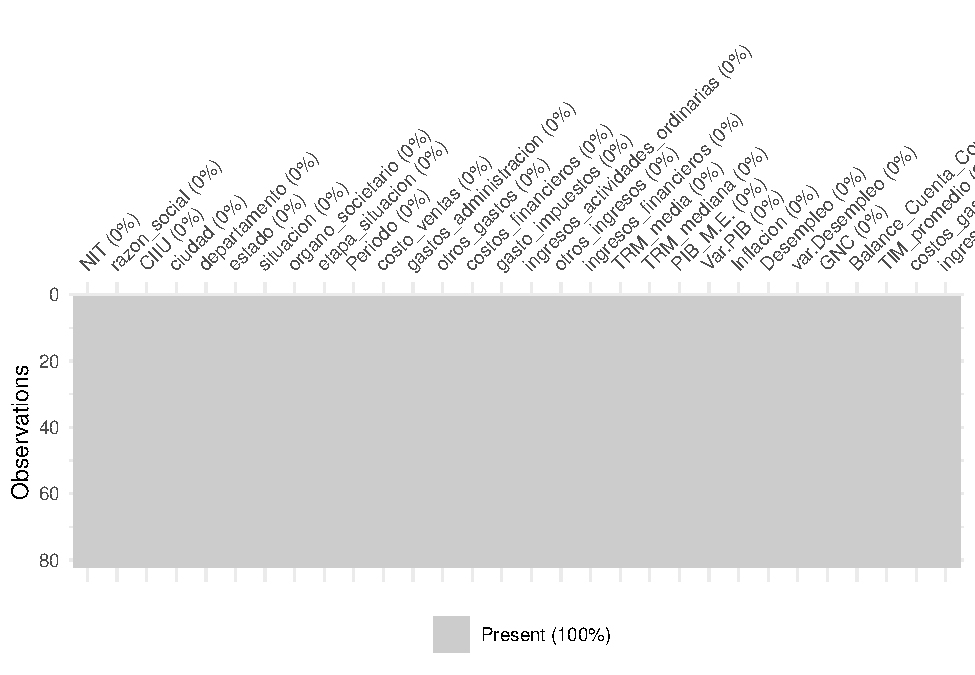
\includegraphics{index_files/figure-latex/unnamed-chunk-4-1.pdf} \#
Capítulo 4: análisis descriptivo

\begin{Shaded}
\begin{Highlighting}[]
\KeywordTok{library}\NormalTok{(ggplot2)}
\KeywordTok{library}\NormalTok{(tidyr)}
\NormalTok{datosValidar <-}\StringTok{ }\NormalTok{base_modelado }\OperatorTok\StringTok{ }\KeywordTok{group_by}\NormalTok{(NIT, razon_social) }\OperatorTok\StringTok{ }\KeywordTok{summarise}\NormalTok{(}\DataTypeTok{total=}\KeywordTok{n}\NormalTok{()) }
\end{Highlighting}
\end{Shaded}

\begin{verbatim}
## `summarise()` regrouping output by 'NIT' (override with `.groups` argument)
\end{verbatim}

\begin{Shaded}
\begin{Highlighting}[]
\CommentTok{#crear histograma para ver la cantidad de periodos por empresa}
\KeywordTok{ggplot}\NormalTok{(datosValidar, }\KeywordTok{aes}\NormalTok{(}\DataTypeTok{x=}\NormalTok{total)) }\OperatorTok{+}\StringTok{ }\KeywordTok{geom_histogram}\NormalTok{()}
\end{Highlighting}
\end{Shaded}

\begin{verbatim}
## `stat_bin()` using `bins = 30`. Pick better value with `binwidth`.
\end{verbatim}

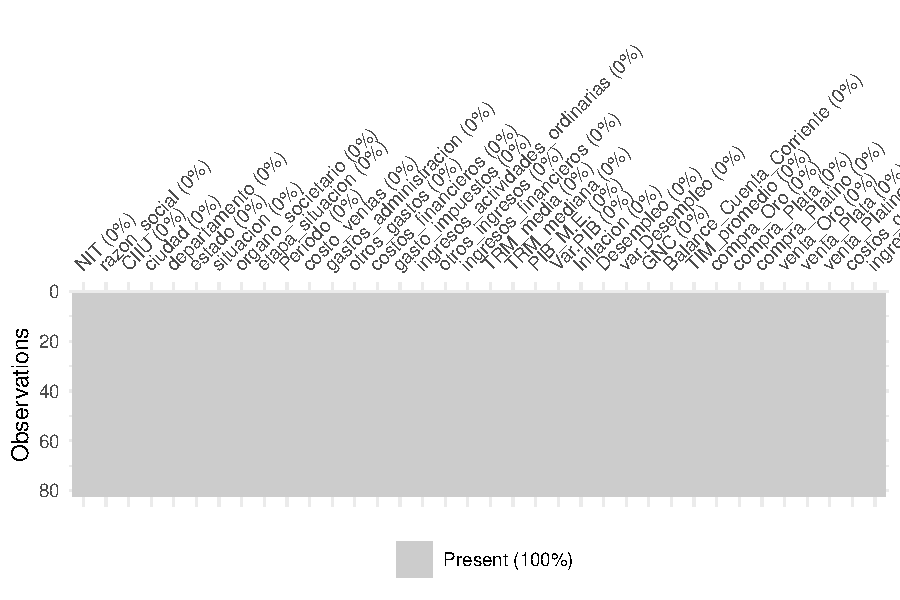
\includegraphics{index_files/figure-latex/unnamed-chunk-5-1.pdf}

\begin{Shaded}
\begin{Highlighting}[]
\NormalTok{datosValidarDepartamento <-}\StringTok{ }\NormalTok{base_modelado }\OperatorTok\StringTok{ }\KeywordTok{group_by}\NormalTok{(departamento, Periodo) }\OperatorTok\StringTok{ }\KeywordTok{summarise}\NormalTok{(}\DataTypeTok{costo_gasto_total_dep =} \KeywordTok{sum}\NormalTok{(costos_gastos_totales) }\OperatorTok{/}\StringTok{ }\DecValTok{1000000}\NormalTok{,}
                                                                                           \DataTypeTok{ingresos_totales_dep =} \KeywordTok{sum}\NormalTok{(ingresos_totales) }\OperatorTok{/}\StringTok{ }\DecValTok{1000000}\NormalTok{)}
\end{Highlighting}
\end{Shaded}

\begin{verbatim}
## `summarise()` regrouping output by 'departamento' (override with `.groups` argument)
\end{verbatim}

\begin{Shaded}
\begin{Highlighting}[]
\KeywordTok{ggplot}\NormalTok{(datosValidarDepartamento, }\KeywordTok{aes}\NormalTok{(}\DataTypeTok{x=}\NormalTok{ Periodo))}\OperatorTok{+}
\StringTok{  }\KeywordTok{geom_line}\NormalTok{(}\KeywordTok{aes}\NormalTok{(}\DataTypeTok{y =}\NormalTok{ costo_gasto_total_dep), }\DataTypeTok{color=}\StringTok{"darkred"}\NormalTok{, }\DataTypeTok{linetype=}\StringTok{"twodash"}\NormalTok{)}\OperatorTok{+}
\StringTok{  }\KeywordTok{geom_label}\NormalTok{(}\KeywordTok{aes}\NormalTok{(}\DataTypeTok{y =}\NormalTok{ costo_gasto_total_dep, }\DataTypeTok{label=}\NormalTok{costo_gasto_total_dep)) }\OperatorTok{+}\StringTok{ }
\StringTok{  }\KeywordTok{geom_line}\NormalTok{(}\KeywordTok{aes}\NormalTok{(}\DataTypeTok{y =}\NormalTok{ ingresos_totales_dep, }\DataTypeTok{label=}\StringTok{"Ingresos"}\NormalTok{), }\DataTypeTok{color =} \StringTok{"steelblue"}\NormalTok{)}\OperatorTok{+}
\StringTok{  }\KeywordTok{geom_label}\NormalTok{(}\KeywordTok{aes}\NormalTok{(}\DataTypeTok{y =}\NormalTok{ ingresos_totales_dep, }\DataTypeTok{label=}\NormalTok{ingresos_totales_dep)) }\OperatorTok{+}\StringTok{ }
\StringTok{  }\KeywordTok{facet_wrap}\NormalTok{(}\OperatorTok{~}\NormalTok{departamento, }\DataTypeTok{scales =}\StringTok{"free_y"}\NormalTok{)}
\end{Highlighting}
\end{Shaded}

\begin{verbatim}
## Warning: Ignoring unknown aesthetics: label
\end{verbatim}

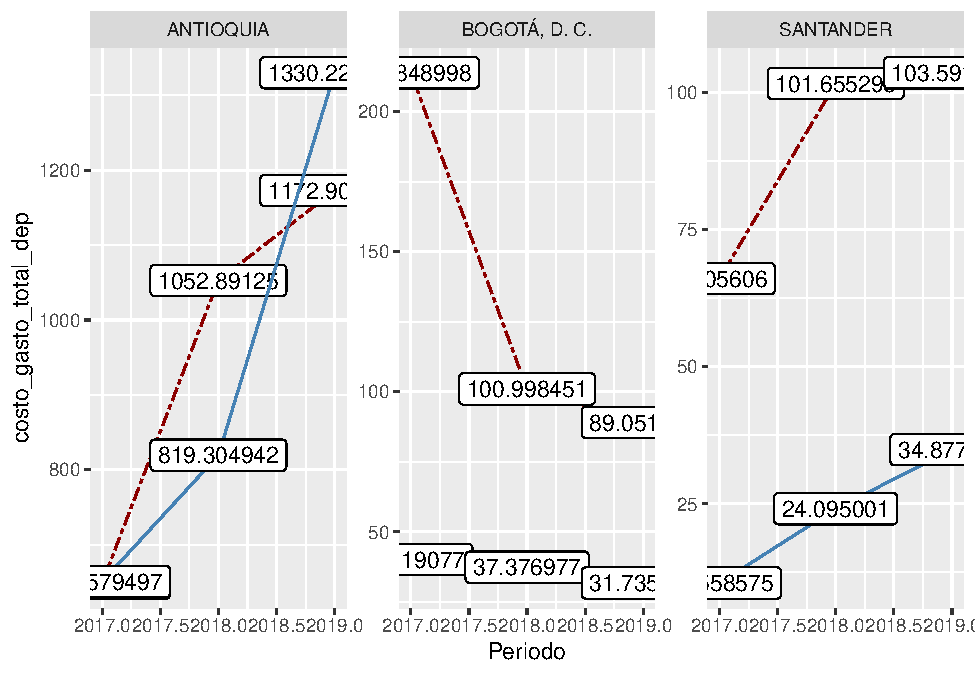
\includegraphics{index_files/figure-latex/unnamed-chunk-5-2.pdf}

\end{document}
